\newpage
\pagestyle{fancy}
\lhead{\textsc{Chapitre 5. Conception et mise en œuvre de l'application décisionnelle prédictive}}
\renewcommand{\headrulewidth}{0.5pt}
\renewcommand{\footrulewidth}{0.5pt}

\chapter{Conception et mise en œuvre de l'application décisionnelle prédictive BIOSPHERE}\setlength{\headheight}{28pt}
\label{ch5}
\minitoc
\newpage

\section{Introduction}

Dans les chapitres précédents, nous avons présenté le contexte du projet, les différentes étapes de préparation des données ainsi que le développement des modèles de Machine Learning destinés à la prédiction des ruptures de stock et à l'estimation des niveaux futurs de stock.

Après la phase de modélisation, la méthodologie CRISP-DM préconise une phase de déploiement visant à rendre les résultats obtenus exploitables par les utilisateurs métier. Cette étape consiste à intégrer les modèles développés dans une solution informatique permettant leur utilisation dans un environnement opérationnel réel.

Dans ce cadre, une application décisionnelle Desktop a été conçue et développée pour l'entreprise BIOSPHERE. Cette application centralise les indicateurs de performance, les résultats des modèles d'intelligence artificielle, les alertes de rupture ainsi que les recommandations de réapprovisionnement afin d'assister les responsables dans leurs prises de décision.

Ce chapitre présente les travaux réalisés lors du Sprint 5 du projet ainsi que la mise en œuvre de la phase de déploiement de la méthodologie CRISP-DM. Il décrit ensuite l'application Desktop développée, ses différents modules fonctionnels, les raisons ayant motivé le choix d'une architecture Desktop ainsi que les aspects techniques liés à son implémentation.

\section{Section 1: Sprint 5 : Intégration finale et système décisionnel intelligent}

\subsection{Objectifs du Sprint 5}

Le Sprint 5 représente la dernière itération du projet BIOSPHERE. Son objectif principal était d'assurer l'intégration complète des modèles d'intelligence artificielle développés lors des sprints précédents au sein d'une plateforme décisionnelle destinée aux utilisateurs finaux.

Ce sprint a permis de transformer les résultats analytiques et prédictifs obtenus à travers les modèles de classification et de régression en outils d'aide à la décision directement exploitables par les responsables métier. Les travaux réalisés se sont concentrés sur la conception de l'interface utilisateur, l'intégration des modèles de Machine Learning, l'automatisation des processus de prédiction ainsi que la génération des alertes intelligentes.

\begin{table}[H]
\centering
\caption{Sprint 5 : Intégration finale et système décisionnel intelligent}
\label{tab:ch5:sprint5}
\small
\begin{tabular}{|p{3.5cm}|p{1.5cm}|p{1.5cm}|p{2.2cm}|p{5.5cm}|}
\hline
\multicolumn{1}{|c|}{\textbf{Sprint}} & 
\multicolumn{1}{c|}{\textbf{User Stories}} & 
\multicolumn{1}{c|}{\textbf{Priorité}} & 
\multicolumn{1}{c|}{\textbf{Durée estimée}} & 
\multicolumn{1}{c|}{\textbf{Livrable attendu}} \\
\hline
Sprint 5 : Application décisionnelle BIOSPHERE Decision System & US02, US03, US05 & Haute & 2 semaines & Application desktop BIOSPHERE Decision System : Authentification sécurisée, intégration des KPI BI, visualisation des prédictions IA, système d'alertes automatisées \\
\hline
\end{tabular}
\end{table}

\subsection{Travaux réalisés}

Le Sprint 5 a été consacré à l'intégration finale des différents composants développés au cours du projet ainsi qu'à la mise en œuvre de l'interface utilisateur destinée aux décideurs de BIOSPHERE.

Dans un premier temps, les résultats issus des modèles de Machine Learning développés lors des sprints précédents ont été intégrés dans une application décisionnelle unique. Cette étape a permis de transformer les résultats analytiques et prédictifs en informations directement exploitables par les utilisateurs métier.

Par la suite, plusieurs modules fonctionnels ont été développés afin de répondre aux besoins identifiés lors de l'analyse métier. Un tableau de bord décisionnel a été conçu pour offrir une vue synthétique des principaux indicateurs de performance. En parallèle, un module Business Intelligence a été intégré afin de permettre le suivi des ventes, des achats, du profit, de la marge et des niveaux de stock.

Le système de prévision des stocks a également été connecté à l'application. Celui-ci exploite les résultats des modèles de classification et de régression afin d'anticiper les risques de rupture et d'estimer les niveaux futurs de stock. Ces prédictions sont ensuite utilisées pour générer automatiquement des recommandations de réapprovisionnement.

Afin d'améliorer la réactivité des utilisateurs face aux situations critiques, un module de gestion des alertes a été développé. Ce dernier permet de détecter automatiquement les produits présentant un risque élevé de rupture et de notifier les responsables concernés.

Enfin, plusieurs fonctionnalités complémentaires ont été ajoutées, notamment l'exportation des résultats, la gestion des utilisateurs selon leurs rôles ainsi que les mécanismes de configuration et d'administration de l'application.

L'ensemble de ces réalisations a permis de disposer d'une solution décisionnelle complète regroupant les fonctionnalités de Business Intelligence et d'intelligence artificielle au sein d'un environnement unique destiné à l'aide à la décision.

\begin{figure}[H]
\centering

\includegraphics[width=0.9\textwidth]{fig62_realisations_sprint5.png}
\caption{Vue d'ensemble des principales réalisations effectuées durant le Sprint 5}
\label{fig:ch5:realisations_sprint5}
\end{figure}

\subsubsection{Authentification et accès à l'application}

La première fonctionnalité réalisée concerne le mécanisme d'authentification permettant de sécuriser l'accès à la plateforme décisionnelle. L'utilisateur doit saisir ses identifiants afin d'accéder aux modules correspondant à son rôle. Cette étape garantit la confidentialité des données et le contrôle des accès au système.

\begin{figure}[H]
\centering

\includegraphics[width=0.7\textwidth]{fig63_connexion.png}
\caption{Interface de connexion de l'application décisionnelle}
\label{fig:ch5:connexion}
\end{figure}

\subsubsection{Administration du système}

Afin d'assurer la gestion, la maintenance et la sécurisation de la plateforme décisionnelle, un module d'administration a été intégré à l'application BIOSPHERE. Cette interface est réservée aux utilisateurs disposant du rôle Administrateur et permet de centraliser l'ensemble des paramètres nécessaires au bon fonctionnement du système.

L'objectif principal de ce module est de fournir un environnement de configuration permettant de gérer les utilisateurs, les paramètres de notification, les seuils décisionnels ainsi que les préférences générales de l'application. Cette centralisation facilite l'administration quotidienne de la solution tout en garantissant un contrôle efficace des accès et des fonctionnalités disponibles.

Le module d'administration est organisé autour de plusieurs sections accessibles depuis un menu latéral :

\begin{itemize}
    \item Gestion des comptes utilisateurs 
    \item Configuration des emails 
    \item Paramétrage des alertes 
    \item Préférences système.
\end{itemize}

La section de gestion des comptes permet à l'administrateur de créer, modifier ou supprimer des utilisateurs. Chaque utilisateur est associé à un rôle spécifique déterminant son niveau d'accès au système. Les rôles implémentés dans l'application sont l'Administrateur, le Directeur, le Manager Tunisie et le Manager Sfax. Les informations relatives aux comptes sont centralisées dans une interface permettant également de consulter leur statut d'activation. Les mots de passe sont stockés sous forme hachée afin de renforcer la sécurité des données d'authentification.

\begin{figure}[H]
\centering

\includegraphics[width=1.1\textwidth]{fig64_admin_users.png}
\caption{Interface Administrateur : Gestion des comptes utilisateurs}
\label{fig:ch5:admin_users}
\end{figure}

La section de configuration des emails permet de paramétrer les destinataires des notifications automatiques générées par le système. Elle affiche les informations du serveur SMTP utilisé pour l'envoi des messages ainsi que les adresses électroniques associées aux différents profils de gestion. Cette fonctionnalité assure la transmission automatique des alertes critiques aux responsables concernés.

\begin{figure}[H]
\centering

\includegraphics[width=0.9\textwidth]{fig65_admin_emails.png}
\caption{Interface d'administration : Configuration des emails}
\label{fig:ch5:admin_emails}
\end{figure}

La section de paramétrage des alertes offre la possibilité de définir les seuils utilisés par le moteur décisionnel pour classifier les risques détectés. L'administrateur peut notamment ajuster les seuils de risque critique, les seuils de risque moyen, les limites de stock ainsi que les paramètres d'envoi automatique des notifications. Cette flexibilité permet d'adapter le comportement du système aux besoins spécifiques de l'entreprise.

\begin{figure}[H]
\centering

\includegraphics[width=1.1\textwidth]{fig66_admin_alertes.png}
\caption{Interface d'administration : Paramétrage des seuils d'alerte}
\label{fig:ch5:admin_alertes}
\end{figure}

Enfin, la section des préférences système regroupe différents paramètres généraux liés au fonctionnement de l'application. Elle fournit des informations sur la version du système, le mode de fonctionnement, les paramètres régionaux ainsi que plusieurs actions de maintenance telles que le nettoyage du cache, le rechargement des données d'intelligence artificielle ou la vérification de l'état général du système.

\begin{figure}[H]
\centering

\includegraphics[width=1.1\textwidth]{fig67_admin_preferences.png}
\caption{Interface d'administration : Préférences système et maintenance}
\label{fig:ch5:admin_preferences}
\end{figure}

\subsubsection{Tableau de bord décisionnel}

Le tableau de bord décisionnel constitue l'écran principal de l'application BIOSPHERE. Il offre aux décideurs une vue synthétique et centralisée des principaux indicateurs de performance ainsi que de l'état global du système d'intelligence artificielle.

Après authentification, l'utilisateur accède à cette interface qui regroupe les informations essentielles nécessaires au suivi de l'activité. Une barre latérale de navigation située à gauche permet d'accéder rapidement aux différents modules de l'application, notamment le module Business Intelligence, le système de prévision des stocks et le module de gestion des alertes.

Dans la partie supérieure de l'interface, plusieurs informations contextuelles sont affichées, notamment le profil de l'utilisateur connecté, son rôle, l'année d'analyse en cours, la date des données exploitées ainsi que la date de la dernière actualisation du système. Des boutons d'accès rapide permettent également de consulter directement les alertes actives ou les prévisions de stock.

Le tableau de bord intègre ensuite une zone de supervision du système d'intelligence artificielle. Cette section informe l'utilisateur de l'état opérationnel des différents composants de la plateforme. Les indicateurs affichent notamment la disponibilité du module Business Intelligence, du moteur d'intelligence artificielle, du système d'alertes et de la connexion aux données. Ces éléments permettent de vérifier rapidement le bon fonctionnement de l'ensemble de la solution décisionnelle.

La partie inférieure de l'interface présente les principaux indicateurs clés de performance (KPI) sous forme de cartes synthétiques. Parmi les indicateurs affichés figurent :

\begin{itemize}
    \item le chiffre d'affaires total réalisé ;
    \item le profit généré ;
    \item le taux de marge commerciale ;
    \item le volume de stock disponible ;
    \item le nombre d'articles en rupture.
\end{itemize}

Chaque indicateur est accompagné de sa valeur détaillée afin de faciliter l'interprétation des résultats par les responsables métiers.

Cette interface joue un rôle central dans le processus décisionnel puisqu'elle permet de visualiser en temps réel l'état de l'activité, les performances commerciales et les informations issues des modèles prédictifs intégrés dans l'application.

\begin{figure}[H]
\centering

\includegraphics[width=1.1\textwidth]{fig68_dashboard.png}
\caption{Tableau de bord décisionnel}
\label{fig:ch5:dashboard}
\end{figure}

\subsubsection{Module Business Intelligence}

Le module Business Intelligence (BI) constitue le centre d'analyse de la performance de l'entreprise au sein de la solution BIOSPHERE. Son objectif est de fournir aux décideurs une vision synthétique et actualisée des principaux indicateurs de gestion afin de faciliter le pilotage de l'activité.

L'interface présente dans sa partie supérieure des informations de contexte permettant d'identifier le périmètre d'analyse, notamment le rôle de l'utilisateur connecté, les sites concernés, l'année d'analyse active, la date des données exploitées ainsi que la date de la dernière mise à jour. Un bouton d'exportation permet également de générer les indicateurs sous format CSV pour une utilisation externe ou des analyses complémentaires.

Le cœur du module est constitué d'un ensemble de cartes de performance (KPI) affichant les indicateurs stratégiques de l'entreprise. Parmi les mesures disponibles figurent :

\begin{itemize}
    \item Le montant total des ventes réalisées 
    \item Le volume des achats effectués 
    \item Le profit généré 
    \item Le taux de marge commerciale 
    \item Le stock total disponible 
    \item Le stock mobilisable 
    \item Le nombre d'articles en rupture
\end{itemize}

Chaque indicateur est présenté sous une forme simplifiée pour une lecture rapide, tout en conservant sa valeur exacte afin de garantir la précision de l'analyse.

Le module intègre également des informations techniques permettant de vérifier la disponibilité des données et l'état du chargement des indicateurs. Ces informations assurent la traçabilité des résultats affichés et facilitent le contrôle du bon fonctionnement du système décisionnel.

Grâce à cette interface, les responsables disposent d'une vision globale de la situation commerciale et logistique de l'entreprise. Les informations présentées permettent d'évaluer rapidement la performance de l'activité, d'identifier les écarts éventuels et de soutenir les décisions stratégiques liées à la gestion des ventes, des achats et des stocks.

\begin{figure}[H]
\centering

\includegraphics[width=1.1\textwidth]{fig69_module_bi.png}
\caption{Interface du module Business Intelligence}
\label{fig:ch5:module_bi}
\end{figure}

\subsubsection{Module de prévision des stocks}

Le système de prévision des stocks exploite les modèles de Machine Learning développés précédemment afin d'identifier les risques de rupture et d'estimer les niveaux futurs de stock. Le processus de prédiction est exécuté automatiquement à travers le moteur d'intelligence artificielle intégré à l'application.

Le module de prévision des stocks constitue le cœur analytique de la solution BIOSPHERE. Il exploite les modèles d'intelligence artificielle développés au cours du projet afin d'anticiper les risques de rupture et d'assister les gestionnaires dans leurs décisions de réapprovisionnement.

L'interface affiche dans sa partie supérieure des informations générales relatives à l'exécution du moteur prédictif, notamment le rôle de l'utilisateur connecté, la source de données utilisée ainsi que la date de la dernière actualisation des résultats. Des fonctionnalités d'exportation permettent également de sauvegarder les résultats des prévisions et les recommandations générées.

Le module intègre un moteur de prédiction intelligent chargé d'exécuter les différentes étapes du processus analytique. Une barre de progression permet de suivre l'état d'avancement des traitements tandis qu'un indicateur visuel confirme l'activation du moteur d'intelligence artificielle.

La section « Processus IA » présente les principales étapes exécutées par le système :

\begin{itemize}
    \item Chargement des données 
    \item Préparation des variables 
    \item Classification du risque de rupture 
    \item Prévision du niveau de stock 
    \item Génération des recommandations de réapprovisionnement
\end{itemize}

Cette représentation permet à l'utilisateur de suivre le déroulement des traitements réalisés par les modèles de Machine Learning avant l'affichage des résultats finaux.

\begin{figure}[H]
\centering

\includegraphics[width=1.1\textwidth]{fig70_moteur_prevision.png}
\caption{Moteur de prévision des stocks}
\label{fig:ch5:moteur_prevision}
\end{figure}
\begin{figure}[H]
\centering

\includegraphics[width=1.1\textwidth]{fig71_suite_prevision.png}
\caption{Suite -- Moteur de prévision des stocks}
\label{fig:ch5:suite_prevision}
\end{figure}

L'objectif principal de ce module est d'identifier de manière proactive les produits susceptibles de connaître une rupture de stock. Les prévisions produites sont ensuite utilisées pour alimenter les mécanismes d'alerte et les recommandations décisionnelles intégrés dans l'application.

\subsubsection{Module de gestion des alertes}

Le module de gestion des alertes permet de surveiller en continu les résultats générés par les modèles d'intelligence artificielle afin d'identifier rapidement les situations nécessitant une intervention. Il constitue un mécanisme d'aide à la décision visant à réduire les risques de rupture de stock et à améliorer la réactivité des gestionnaires.

L'interface présente dans sa partie supérieure un résumé de l'état global du système d'alertes à travers plusieurs indicateurs clés. Ces indicateurs affichent notamment le nombre d'alertes critiques, le nombre d'alertes moyennes, les emails en attente d'envoi ainsi que le nombre total d'alertes actives. Cette synthèse permet aux responsables d'évaluer rapidement le niveau de risque associé aux stocks de l'entreprise.

Le module offre également des fonctionnalités de gestion et de suivi des notifications. Les utilisateurs peuvent générer ou actualiser les alertes à partir des résultats prédictifs, exporter les données au format CSV ou encore effectuer des tests d'envoi d'emails afin de vérifier le bon fonctionnement du système de notification.

Afin de faciliter l'analyse, des filtres de recherche sont disponibles selon plusieurs critères tels que le niveau de priorité, le site concerné ou le produit analysé. Ces fonctionnalités permettent de cibler rapidement les alertes les plus importantes et d'améliorer l'efficacité du suivi opérationnel.

La partie inférieure de l'interface affiche l'historique détaillé des alertes générées par le système. Pour chaque alerte, plusieurs informations sont fournies :

\begin{itemize}
    \item La date de génération 
    \item Le produit concerné 
    \item Le site associé 
    \item Le niveau de priorité 
    \item Le type d'alerte 
    \item La raison de l'alerte 
    \item Le score de risque calculé 
    \item Le stock prévisionnel estimé 
    \item L'explication du risque détecté
\end{itemize}

Ces informations permettent aux décideurs de comprendre l'origine de chaque alerte et de prendre les mesures correctives appropriées.

\begin{figure}[H]
\centering

\includegraphics[width=1.1\textwidth]{fig72_alertes.png}
\caption{Interface de gestion des alertes}
\label{fig:ch5:alertes}
\end{figure}

\section{Section 2 : Déploiement de la solution selon CRISP-DM}

\subsection{Présentation de la phase Déploiement}

La phase de Déploiement (Deployment) constitue la dernière étape de la méthodologie CRISP-DM. Après la compréhension du métier, la préparation des données, la modélisation et l'évaluation des modèles, cette phase vise à rendre les résultats obtenus directement exploitables par les utilisateurs finaux.

Dans le cadre du projet BIOSPHERE, les modèles d'intelligence artificielle développés lors des phases précédentes ont démontré leur capacité à prédire les risques de rupture de stock et à générer des recommandations de réapprovisionnement pertinentes. Toutefois, ces modèles ne peuvent apporter une réelle valeur ajoutée que s'ils sont intégrés dans un environnement accessible aux décideurs.

L'objectif principal de cette phase consiste donc à transformer les résultats analytiques et prédictifs en une solution opérationnelle permettant aux responsables de consulter les indicateurs de performance, d'analyser les prévisions de stock et de gérer les alertes à partir d'une interface unique.

Pour répondre à cet objectif, une application décisionnelle desktop a été développée afin d'assurer l'intégration des différents modules réalisés durant les sprints précédents. Cette application centralise les fonctionnalités de Business Intelligence, les modèles de Machine Learning ainsi que les mécanismes d'alerte dans un environnement cohérent et intuitif.

La phase de déploiement ne se limite donc pas à l'installation technique de la solution. Elle englobe également la conception de l'architecture applicative, l'intégration des composants décisionnels, la mise à disposition des fonctionnalités métiers et la validation du fonctionnement global du système.

Ainsi, cette étape permet de concrétiser l'ensemble des travaux réalisés tout au long du projet en fournissant une plateforme décisionnelle intelligente capable d'assister les gestionnaires dans leurs prises de décision quotidiennes.

\begin{table}[H]
\centering
\caption{Position de la phase Déploiement dans le cycle CRISP-DM}
\label{tab:ch5:deployment_crisp}
\small
\begin{tabular}{|p{4cm}|p{5.5cm}|p{5.5cm}|}
\hline
\multicolumn{1}{|c|}{\textbf{Phase CRISP-DM}} & 
\multicolumn{1}{c|}{\textbf{Objectif}} & 
\multicolumn{1}{c|}{\textbf{Livrable}} \\
\hline
Phase 6 : Déploiement & Intégrer les modèles dans l'environnement décisionnel & Application décisionnelle enrichie par l'IA \\
\hline
\end{tabular}
\end{table}

\subsection{Choix de l'application Desktop}

Dans le cadre de la phase de déploiement, plusieurs solutions de mise à disposition du système décisionnel ont été envisagées, principalement les applications web et les applications desktop.

Après analyse des besoins du projet et des contraintes techniques, le choix s'est porté sur le développement d'une application desktop.

Ce choix s'explique par la nécessité de centraliser les différents composants du système décisionnel dans un environnement unique capable d'interagir directement avec les sources de données, les résultats des modèles de Machine Learning et les différents modules métiers. L'application desktop permet ainsi de fournir une solution autonome, facilement exécutable sur les postes des utilisateurs sans nécessiter d'infrastructure web complexe.

Par ailleurs, l'environnement de développement du projet repose essentiellement sur l'écosystème Python. Les modèles de prédiction des stocks, les traitements analytiques ainsi que les différents services applicatifs ont été développés dans ce langage.

L'application développée offre également une meilleure maîtrise de l'architecture du système. L'ensemble des fonctionnalités est regroupé au sein d'une interface unique comprenant un module d'authentification, un tableau de bord décisionnel, un espace Business Intelligence, un module de prévision des stocks, un système de gestion des alertes ainsi qu'un espace d'administration réservé aux administrateurs.

Contrairement à une application web qui nécessite généralement un serveur applicatif, une gestion du déploiement réseau et des mécanismes de sécurité supplémentaires, l'application desktop permet une mise en œuvre plus simple tout en répondant efficacement aux besoins fonctionnels du projet. Cette approche réduit également les dépendances vis-à-vis des services externes et facilite les démonstrations ainsi que les tests en environnement local.

Enfin, le choix de l'interface graphique CustomTkinter a permis de concevoir une application moderne, ergonomique et adaptée à la consultation des indicateurs décisionnels. Cette technologie offre une expérience utilisateur fluide tout en restant légère et compatible avec l'environnement Python utilisé dans le projet.

\begin{table}[H]
\centering
\caption{Comparaison entre une application Web et une application Desktop dans le contexte du projet BIOSPHERE}
\label{tab:ch5:web_vs_desktop}
\small
\begin{tabular}{|p{3.5cm}|p{5cm}|p{5.5cm}|}
\hline
\multicolumn{1}{|c|}{\textbf{Critère}} & \multicolumn{1}{c|}{\textbf{Application Web}} & \multicolumn{1}{c|}{\textbf{Application Desktop BIOSPHERE}} \\
\hline
Déploiement & Nécessite un serveur web et une infrastructure réseau & Installation directe sur le poste utilisateur \\
\hline
Connexion Internet & Généralement requise & Fonctionnement local possible \\
\hline
Intégration avec Python & Nécessite souvent une couche supplémentaire (API, Backend Web) & Intégration directe des modèles IA Python \\
\hline
Complexité de développement & Plus élevée (Frontend + Backend + Hébergement) & Plus simple dans le contexte du projet \\
\hline
Maintenance & Dépend du serveur et des services déployés & Maintenance locale simplifiée \\
\hline
Sécurité & Gestion des accès réseau et du serveur & Exécution locale avec contrôle des utilisateurs \\
\hline
Performance & Dépend du réseau et du serveur & Exécution directe sur la machine \\
\hline
Accès aux données locales & Limité & Accès direct aux fichiers et ressources locales \\
\hline
Intégration SQL Server & Via services intermédiaires & Connexion directe \\
\hline
Adaptation aux besoins du projet & Partiellement adaptée & Totalement adaptée \\
\hline
\end{tabular}
\end{table}

L'analyse comparative présentée dans le tableau précédent montre que l'approche desktop répond davantage aux exigences du projet BIOSPHERE. En effet, cette solution permet une intégration directe des modèles d'intelligence artificielle développés en Python, une connexion simplifiée au Data Warehouse SQL Server ainsi qu'une exécution locale indépendante d'une infrastructure web complexe. Ces caractéristiques ont conduit au choix d'une application desktop comme support de déploiement de la plateforme décisionnelle prédictive.

\subsection{Architecture fonctionnelle}

L'architecture fonctionnelle de l'application BIOSPHERE a été conçue afin de centraliser les différentes fonctionnalités décisionnelles développées durant le projet au sein d'une plateforme unique. Elle permet aux utilisateurs métiers d'accéder aux informations stratégiques, aux prévisions de stock et aux alertes de manière simple et structurée.

Le fonctionnement général de l'application repose sur une authentification préalable de l'utilisateur. Après connexion, les fonctionnalités accessibles sont déterminées en fonction du rôle attribué à l'utilisateur.

L'application distingue quatre profils d'utilisateurs :

\begin{itemize}
    \item \textbf{Administrateur (Admin)} : responsable de la configuration de l'application, de la gestion des comptes utilisateurs, des paramètres d'alerte et des paramètres système.
    
    \item \textbf{Directeur} : dispose d'un accès complet aux modules décisionnels et à l'ensemble des données de l'entreprise.
    
    \item \textbf{Manager Tunis (Manager\_TN)} : accède aux informations décisionnelles relatives au site de Tunis.
    
    \item \textbf{Manager Sfax (Manager\_SFX)} : accède aux informations décisionnelles correspondant au site du Sfax.
\end{itemize}

Une fois authentifié, l'utilisateur peut accéder aux différents modules fonctionnels de l'application :

\begin{enumerate}
    \item Le premier module correspond au Dashboard décisionnel. Il constitue le point d'entrée principal de l'application et fournit une vue synthétique de la situation de l'entreprise. Ce tableau de bord regroupe les indicateurs clés de performance, l'état du système d'intelligence artificielle, les alertes critiques ainsi qu'un résumé des prévisions de stock.
    
    \item Le deuxième module est consacré à la Business Intelligence (BI). Il permet de consulter les principaux indicateurs de performance calculés à partir du Data Warehouse de l'entreprise. Les utilisateurs peuvent notamment suivre les ventes, les achats, les profits, les marges, les niveaux de stock ainsi que les articles en rupture.
    
    \item Le troisième module concerne la Prévision des stocks. Ce module exploite les résultats des modèles de Machine Learning développés lors des phases précédentes du projet. Il combine les résultats de classification des risques de rupture avec les prédictions quantitatives de stock afin d'identifier les produits critiques et de proposer des recommandations de réapprovisionnement.
    
    \item Le quatrième module correspond au système de gestion des alertes. Il transforme les résultats des prévisions en alertes métier directement exploitables par les responsables. Les alertes sont classées selon leur niveau de criticité afin de faciliter la priorisation des actions à entreprendre.
\end{enumerate}

Enfin, le module Administration est réservé aux administrateurs. Il permet la gestion des comptes utilisateurs, la configuration des seuils d'alerte, la gestion des destinataires des notifications et l'administration générale de l'application.

Cette organisation fonctionnelle assure une intégration cohérente des différents composants du système décisionnel tout en facilitant la navigation et l'exploitation des résultats analytiques par les utilisateurs métiers.

\subsection{Outils et technologies utilisés}

La réalisation de l'application décisionnelle prédictive BIOSPHERE a nécessité l'utilisation de plusieurs technologies couvrant les différentes couches du système, depuis l'acquisition des données jusqu'à la visualisation des résultats décisionnels.

Le choix de ces outils a été guidé par des critères de performance, de compatibilité avec l'environnement existant de l'entreprise et de facilité d'intégration des modèles d'intelligence artificielle développés durant les phases précédentes du projet.

La couche de développement applicatif a été implémentée en langage Python, qui constitue le cœur de la solution grâce à sa richesse en bibliothèques dédiées à la science des données, au Machine Learning et au développement d'interfaces graphiques. Ce langage a permis d'intégrer efficacement les différents modules analytiques et décisionnels au sein d'une même plateforme.

Pour le développement de l'interface utilisateur, la bibliothèque CustomTkinter a été utilisée afin de concevoir une interface graphique moderne, ergonomique et adaptée aux besoins des utilisateurs métiers. Cette bibliothèque offre une amélioration significative de l'apparence visuelle des interfaces Tkinter traditionnelles tout en conservant leur simplicité de déploiement.

La gestion et l'exploitation des données reposent sur Microsoft SQL Server, qui constitue la source principale des données commerciales, des informations de stock et des historiques de vente. L'accès à la base de données est assuré à travers le connecteur PyODBC permettant l'exécution sécurisée des requêtes SQL depuis l'application.

Les traitements analytiques et statistiques sont réalisés à l'aide des bibliothèques Pandas et NumPy. Ces outils permettent la manipulation, le nettoyage et la transformation des données nécessaires aux modèles d'intelligence artificielle.

Les modèles prédictifs intégrés dans la solution ont été développés à l'aide des bibliothèques Scikit-Learn et XGBoost. Ces frameworks ont permis la mise en œuvre des algorithmes de classification des risques de rupture ainsi que des modèles de régression destinés à la prévision des niveaux de stock futurs.

Le système de visualisation et de reporting s'appuie sur Matplotlib, utilisé pour générer les représentations graphiques intégrées aux modules décisionnels. Ces visualisations facilitent l'interprétation des indicateurs clés de performance et des résultats prédictifs.

Enfin, les mécanismes de notification et d'alerte automatique utilisent les protocoles SMTP pour l'envoi d'emails aux responsables concernés lorsqu'un risque de rupture de stock est détecté.

\begin{small}
\begin{longtable}{|p{2.5cm}|p{2.5cm}|p{4cm}|p{5.5cm}|}
\caption{Outils et technologies utilisés} \label{tab:ch5:outils_technologies} \\
\hline
\multicolumn{1}{|c|}{\textbf{Catégorie}} & 
\multicolumn{1}{c|}{\textbf{Technologie}} & 
\multicolumn{1}{c|}{\textbf{Rôle dans la solution}} & 
\multicolumn{1}{c|}{\textbf{Justification du choix}} \\
\hline
\endhead

\hline
\endfoot

Langage de programmation & Python & Développement global de l'application et intégration des modèles IA & Langage riche en bibliothèques de Data Science, Machine Learning et développement d'interfaces graphiques. \\
\hline
Interface graphique & CustomTkinter & Conception de l'application Desktop & Permet de créer une interface moderne, ergonomique et facilement déployable sans navigateur web. \\
\hline
Base de données & Microsoft SQL Server & Stockage et gestion des données commerciales et de stock & Solution déjà utilisée dans l'environnement BIOSPHERE, fiable et adaptée aux volumes de données traités. \\
\hline
Connectivité BD & PyODBC & Connexion entre Python et SQL Server & Assure une communication stable et sécurisée avec la base de données. \\
\hline
Manipulation des données & Pandas & Nettoyage, transformation et analyse des données & Bibliothèque de référence pour le traitement de données tabulaires en Python. \\
\hline
Calcul numérique & NumPy & Calculs statistiques et opérations matricielles & Optimise les traitements numériques nécessaires aux modèles prédictifs. \\
\hline
Classification ML & Scikit-Learn & Modèle de classification du risque de rupture & Fournit des algorithmes performants et simples à intégrer dans une application métier. \\
\hline
Régression ML & XGBoost & Prévision des niveaux de stock futurs & Offre une excellente précision pour les problèmes de prédiction et de régression. \\
\hline
Visualisation & Matplotlib & Génération des graphiques et indicateurs visuels & Bibliothèque robuste permettant de produire des visualisations personnalisées. \\
\hline
Gestion des alertes & SMTP / smtplib & Envoi automatique des emails d'alerte & Solution standard et légère pour l'automatisation des notifications. \\
\hline
Configuration & JSON & Stockage des paramètres administratifs et seuils d'alerte & Format simple, lisible et facilement modifiable sans intervention sur le code. \\
\hline
Gestion temporelle & Datetime & Manipulation des dates et périodes de prévision & Bibliothèque native Python adaptée aux calculs temporels. \\
\hline
Environnement de développement & Visual Studio Code & Développement et maintenance du projet & IDE léger, performant et compatible avec l'ensemble des technologies utilisées. \\
\hline
Contrôle de version & Git & Suivi des modifications du code source & Facilite la gestion des versions et la collaboration durant le projet. \\
\hline
\end{longtable}
\end{small}

\subsection{Architecture technique}

L'architecture technique de la solution BIOSPHERE a été conçue selon une approche modulaire permettant de séparer les différentes responsabilités du système tout en assurant une communication fluide entre les composants. Cette organisation facilite la maintenance, l'évolution de l'application ainsi que l'intégration des modèles d'intelligence artificielle développés durant les précédents sprints.

L'application repose sur une architecture multicouche composée de quatre niveaux principaux : la couche présentation, la couche métier, la couche analytique et la couche de données.

\begin{figure}[H]
\centering

\includegraphics[width=0.9\textwidth]{fig73_architecture_technique.png}
\caption{L'architecture technique de la solution BIOSPHERE}
\label{fig:ch5:architecture_technique}
\end{figure}

\subsubsection{Couche présentation (Interface utilisateur)}

La couche présentation correspond à l'interface graphique développée avec PySide6. Elle constitue le point d'interaction entre les utilisateurs et le système décisionnel.

Cette couche regroupe l'ensemble des fenêtres et modules de l'application :

\begin{itemize}
    \item Authentification et gestion des rôles 
    \item Tableau de bord décisionnel 
    \item Module Business Intelligence 
    \item Module de prévision des stocks 
    \item Module de gestion des alertes 
    \item Module d'administration
\end{itemize}

L'interface est responsable de l'affichage des indicateurs, des graphiques, des recommandations et des alertes générées par les modèles d'intelligence artificielle.

\begin{figure}[H]
\centering
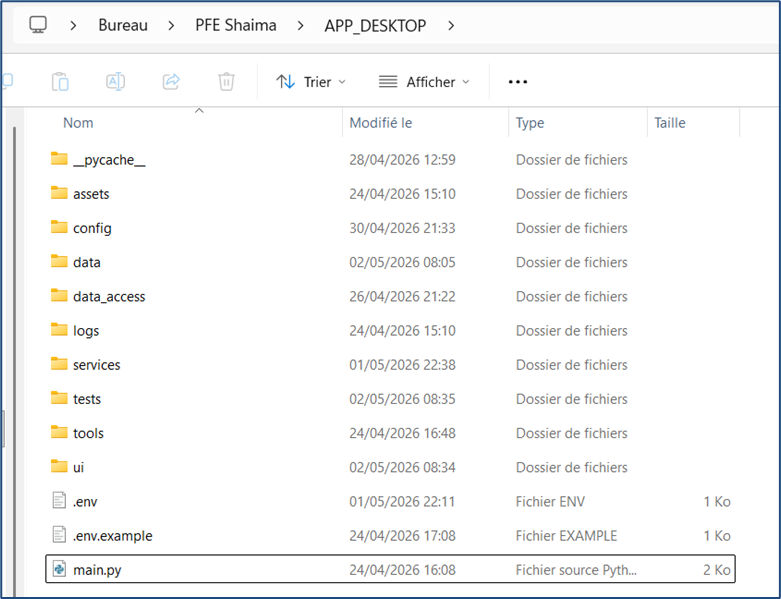
\includegraphics[width=0.7\textwidth]{Figures/Chapitre5/image7.png}
\caption{Structure générale du projet de l'application décisionnelle}
\label{fig:Structure générale du projet de l'application décisionnelle}
\end{figure}

\subsubsection{Couche analytique (Intelligence Artificielle)}

La couche analytique intègre les modèles de Machine Learning développés durant le projet.

Elle comprend :

\begin{itemize}
    \item Le modèle de classification des risques de rupture 
    \item Le modèle de régression de prévision du stock 
    \item Le moteur de génération des recommandations 
    \item Le système d'évaluation des risques
\end{itemize}

À partir des données de stock et des historiques de vente, cette couche produit automatiquement :

\begin{itemize}
    \item Les probabilités de rupture 
    \item Les stocks prévisionnels 
    \item Les niveaux de priorité 
    \item Les recommandations de réapprovisionnement
\end{itemize}

Les résultats générés sont ensuite transmis aux modules décisionnels de l'application.

\subsubsection{Couche métier (Business Layer)}

La couche métier centralise l'ensemble des traitements fonctionnels de l'application. Elle assure la coordination entre l'interface graphique, les modèles d'intelligence artificielle et les données.

Les principales responsabilités de cette couche sont :

\begin{itemize}
    \item Gestion des utilisateurs et des rôles 
    \item Contrôle des accès 
    \item Gestion des indicateurs BI 
    \item Génération des tableaux de bord 
    \item Gestion des alertes 
    \item Configuration système 
    \item Pilotage des processus de prévision
\end{itemize}

Cette couche garantit également la cohérence des informations affichées aux différents profils utilisateurs.

\subsubsection{Couche données}

La couche données assure le stockage et la gestion des informations utilisées par l'application.

Elle comprend :

\begin{itemize}
    \item Les fichiers de données de l'entreprise 
    \item Les fichiers de configuration 
    \item Les modèles IA sauvegardés 
    \item Les paramètres d'administration 
    \item Les historiques d'alertes
\end{itemize}

Les bibliothèques Pandas et NumPy sont utilisées pour le traitement et la manipulation des données avant leur exploitation par les algorithmes de Machine Learning.

\subsubsection{Flux de fonctionnement global}

Le fonctionnement global du système suit les étapes suivantes :

\begin{enumerate}
    \item L'utilisateur s'authentifie à travers l'interface graphique.
    \item Les données sont chargées depuis les sources de stockage.
    \item Les modèles de Machine Learning analysent les données disponibles.
    \item Les prédictions de stock et les scores de risque sont générés.
    \item Le moteur de recommandations produit les actions de réapprovisionnement.
    \item Les résultats sont affichés dans les modules BI, Prévision Stock et Alertes.
    \item Les responsables prennent leurs décisions à partir des informations fournies par le système.
\end{enumerate}

Cette architecture permet de transformer les données opérationnelles en informations décisionnelles exploitables, tout en garantissant une séparation claire entre l'interface utilisateur, la logique métier, les modèles analytiques et les données.


\subsection{Tests fonctionnels réalisés}

Les principaux scénarios de test exécutés sont présentés dans le tableau suivant:

\begin{table}[H]
\centering
\caption{Résultats des tests fonctionnels}
\label{tab:ch5:tests_fonctionnels}
\resizebox{\textwidth}{!}{
\begin{tabular}{|p{3cm}|p{3cm}|p{2.5cm}|p{2.5cm}|p{1.5cm}|}
\hline
\multicolumn{1}{|c|}{\textbf{Fonctionnalité}} & 
\multicolumn{1}{c|}{\textbf{Cas de test}} & 
\multicolumn{1}{c|}{\textbf{Résultat attendu}} & 
\multicolumn{1}{c|}{\textbf{Résultat obtenu}} & 
\multicolumn{1}{c|}{\textbf{Statut}} \\
\hline
Authentification & Connexion avec identifiants valides & Accès à l'application & Accès accordé & Validé \\
\hline
Authentification & Connexion avec identifiants invalides & Refus de connexion & Message d'erreur affiché & Validé \\
\hline
Gestion des rôles & Connexion Manager\_TN & Accès limité au site Tunis & Accès conforme & Validé \\
\hline
Dashboard & Chargement des KPI & Affichage des indicateurs & KPI affichés correctement & Validé \\
\hline
Module BI & Consultation des indicateurs & Affichage des ventes et stocks & Données affichées & Validé \\
\hline
Prévision des stocks & Exécution du moteur IA & Génération des prédictions & Prédictions générées & Validé \\
\hline
Alertes & Détection d'un risque élevé & Création d'une alerte critique & Alerte créée & Validé \\
\hline
Notifications & Envoi d'un email & Réception du message & Email reçu & Validé \\
\hline
Export CSV & Export des résultats & Création du fichier CSV & Fichier généré & Validé \\
\hline
\end{tabular}
}
\end{table}

Les résultats obtenus montrent que l'ensemble des fonctionnalités principales de l'application répond aux exigences fonctionnelles définies lors de l'étude des besoins.

Une attention particulière a été accordée à la validation des modèles de Machine Learning intégrés dans la solution.

Les tests réalisés ont permis de vérifier :

\begin{itemize}
    \item Le chargement correct des modèles sauvegardés 
    \item L'exécution des prédictions à partir des nouvelles données 
    \item La cohérence des résultats affichés dans l'interface 
    \item La génération automatique des recommandations de réapprovisionnement 
    \item La transmission des résultats vers le système d'alertes
\end{itemize}

Les prédictions produites par les modèles sont automatiquement exploitées par le moteur décisionnel afin d'identifier les produits à risque et de proposer les actions correctives adaptées.

Une phase de validation a été réalisée avec les responsables métier de l'entreprise BIOSPHERE afin d'évaluer l'utilisabilité de l'application et la pertinence des informations fournies.

Les utilisateurs ont particulièrement apprécié :

\begin{itemize}
    \item La centralisation des indicateurs au sein d'une interface unique ;
    \item La visualisation des risques de rupture 
    \item L'automatisation des alertes 
    \item La génération des recommandations de réapprovisionnement 
    \item La simplicité de navigation entre les différents modules
\end{itemize}

Les retours obtenus confirment que la solution développée répond aux besoins opérationnels liés à la gestion prévisionnelle des stocks.

L'ensemble des tests réalisés a permis de confirmer la stabilité et le bon fonctionnement de l'application décisionnelle BIOSPHERE. Les différents modules communiquent correctement entre eux et les modèles prédictifs sont intégrés avec succès au sein de la plateforme.

Les résultats obtenus démontrent que la solution est capable de transformer les données opérationnelles en informations décisionnelles exploitables, tout en fournissant aux gestionnaires des outils leur permettant d'anticiper les risques de rupture et d'améliorer la gestion des stocks.

\subsection{Limites de la solution développée}

Malgré les fonctionnalités avancées intégrées à la plateforme décisionnelle BIOSPHERE, certaines limites subsistent et ouvrent la voie à de futures améliorations.

Tout d'abord, la solution a été développée sous la forme d'une application desktop. Bien que ce choix offre de bonnes performances, une meilleure sécurité des données locales et une simplicité de déploiement au sein de l'entreprise, il limite l'accessibilité de l'application. Les utilisateurs doivent disposer d'un poste de travail sur lequel l'application est installée, ce qui ne permet pas un accès distant aussi flexible qu'une application web.

Par ailleurs, l'utilisation simultanée par plusieurs utilisateurs reste dépendante de l'infrastructure de partage des données mise en place. Une architecture web centralisée permettrait de faciliter davantage la collaboration et l'accès aux informations en temps réel depuis différents sites géographiques.

La solution actuelle repose également sur des modèles de Machine Learning entraînés à partir des données historiques disponibles. La qualité des prédictions demeure donc fortement liée à la qualité, à la quantité et à l'actualité des données utilisées. Toute évolution significative du comportement des ventes ou des stocks peut nécessiter un réentraînement périodique des modèles afin de maintenir leur niveau de performance.

De plus, le système de prévision se concentre principalement sur l'analyse des données internes de l'entreprise. L'intégration de données externes telles que les tendances du marché, la saisonnalité avancée, les événements économiques ou les variations de la demande pourrait améliorer davantage la précision des prévisions.

Enfin, bien que le système propose des alertes automatiques et des recommandations de réapprovisionnement, la décision finale demeure sous la responsabilité des gestionnaires. Les recommandations générées doivent être considérées comme une aide à la décision et non comme une automatisation complète du processus de gestion des stocks.

Ces limites constituent autant de perspectives d'amélioration pouvant être explorées dans le cadre de futurs travaux afin de renforcer les capacités analytiques, prédictives et collaboratives de la plateforme.

\section{Conclusion}

Au cours de ce chapitre, nous avons présenté la phase finale du projet consacrée à la conception, au développement et au déploiement de la plateforme décisionnelle prédictive BIOSPHERE. Cette étape a permis de concrétiser l'ensemble des travaux réalisés dans les phases précédentes en intégrant les modèles de Machine Learning développés dans une solution opérationnelle destinée aux utilisateurs métier.

Dans un premier temps, les réalisations du Sprint 5 ont permis la mise en place d'une application décisionnelle complète regroupant les principales fonctionnalités nécessaires au pilotage de l'activité. L'intégration des indicateurs de Business Intelligence, des modèles de prédiction des ruptures de stock, du système de recommandations et du mécanisme d'alertes automatiques a permis de centraliser l'information décisionnelle au sein d'une interface unique, ergonomique et sécurisée.

Dans un second temps, la phase de déploiement de la méthodologie CRISP-DM a été mise en œuvre afin de transformer les résultats analytiques obtenus en un outil directement exploitable par les décideurs. Les choix technologiques adoptés, l'architecture fonctionnelle et l'architecture technique retenues ont permis de garantir l'intégration cohérente des différentes composantes du système tout en assurant sa maintenabilité, sa performance et son évolutivité.

Les tests réalisés ont confirmé le bon fonctionnement des différents modules de la plateforme ainsi que l'intégration effective des modèles prédictifs dans le processus décisionnel. Grâce à l'exploitation conjointe des techniques de Business Intelligence et de Machine Learning, la solution développée permet non seulement d'analyser la situation actuelle des stocks, mais également d'anticiper les risques futurs de rupture et de proposer des actions de réapprovisionnement adaptées.

Ainsi, ce projet a démontré l'intérêt de l'application des approches de Data Science à la gestion des stocks et à l'aide à la décision. La plateforme BIOSPHERE constitue un véritable système décisionnel intelligent capable de transformer les données opérationnelles en connaissances exploitables, contribuant ainsi à l'amélioration de la performance logistique et à l'optimisation des processus de gestion de l'entreprise.

Au-delà des résultats obtenus, cette expérience a permis de mettre en pratique l'ensemble des étapes d'un projet Data Science, depuis la compréhension du besoin métier jusqu'au déploiement d'une solution prédictive en environnement réel. Elle illustre la manière dont les technologies d'intelligence artificielle peuvent être intégrées au sein des systèmes d'information pour soutenir efficacement la prise de décision stratégique et opérationnelle.

